\documentclass[10pt,a4paper]{article}
\usepackage[UTF8]{ctex}
\usepackage{fontspec}
\usepackage{geometry} 
\usepackage{amsmath}
\usepackage[shortlabels]{enumitem}
\usepackage{float}
\usepackage{graphicx}
\usepackage{subfigure}
\usepackage{epstopdf}
\usepackage{amsmath,amssymb}
\usepackage{diagbox}
\usepackage{setspace}
\usepackage{enumitem}
\DeclareSymbolFont{EulerExtension}{U}{euex}{m}{n}
\DeclareMathSymbol{\euintop}{\mathop} {EulerExtension}{"52}
\DeclareMathSymbol{\euointop}{\mathop} {EulerExtension}{"48}
\let\intop\euintop
\let\ointop\euointop

\geometry{left=3.17cm,right=3.17cm,top=2.53cm,bottom=2.54cm}
%\setmainfont{Times New Roman}
\pagestyle{plain}
\setlist[enumerate,1]{label=\textbf{\arabic*.}}
\setlist[enumerate,2]{label=(\arabic*)}

\begin{document}

\begin{enumerate}


    % \begin{figure}[H]
    %     \flushright 
    %     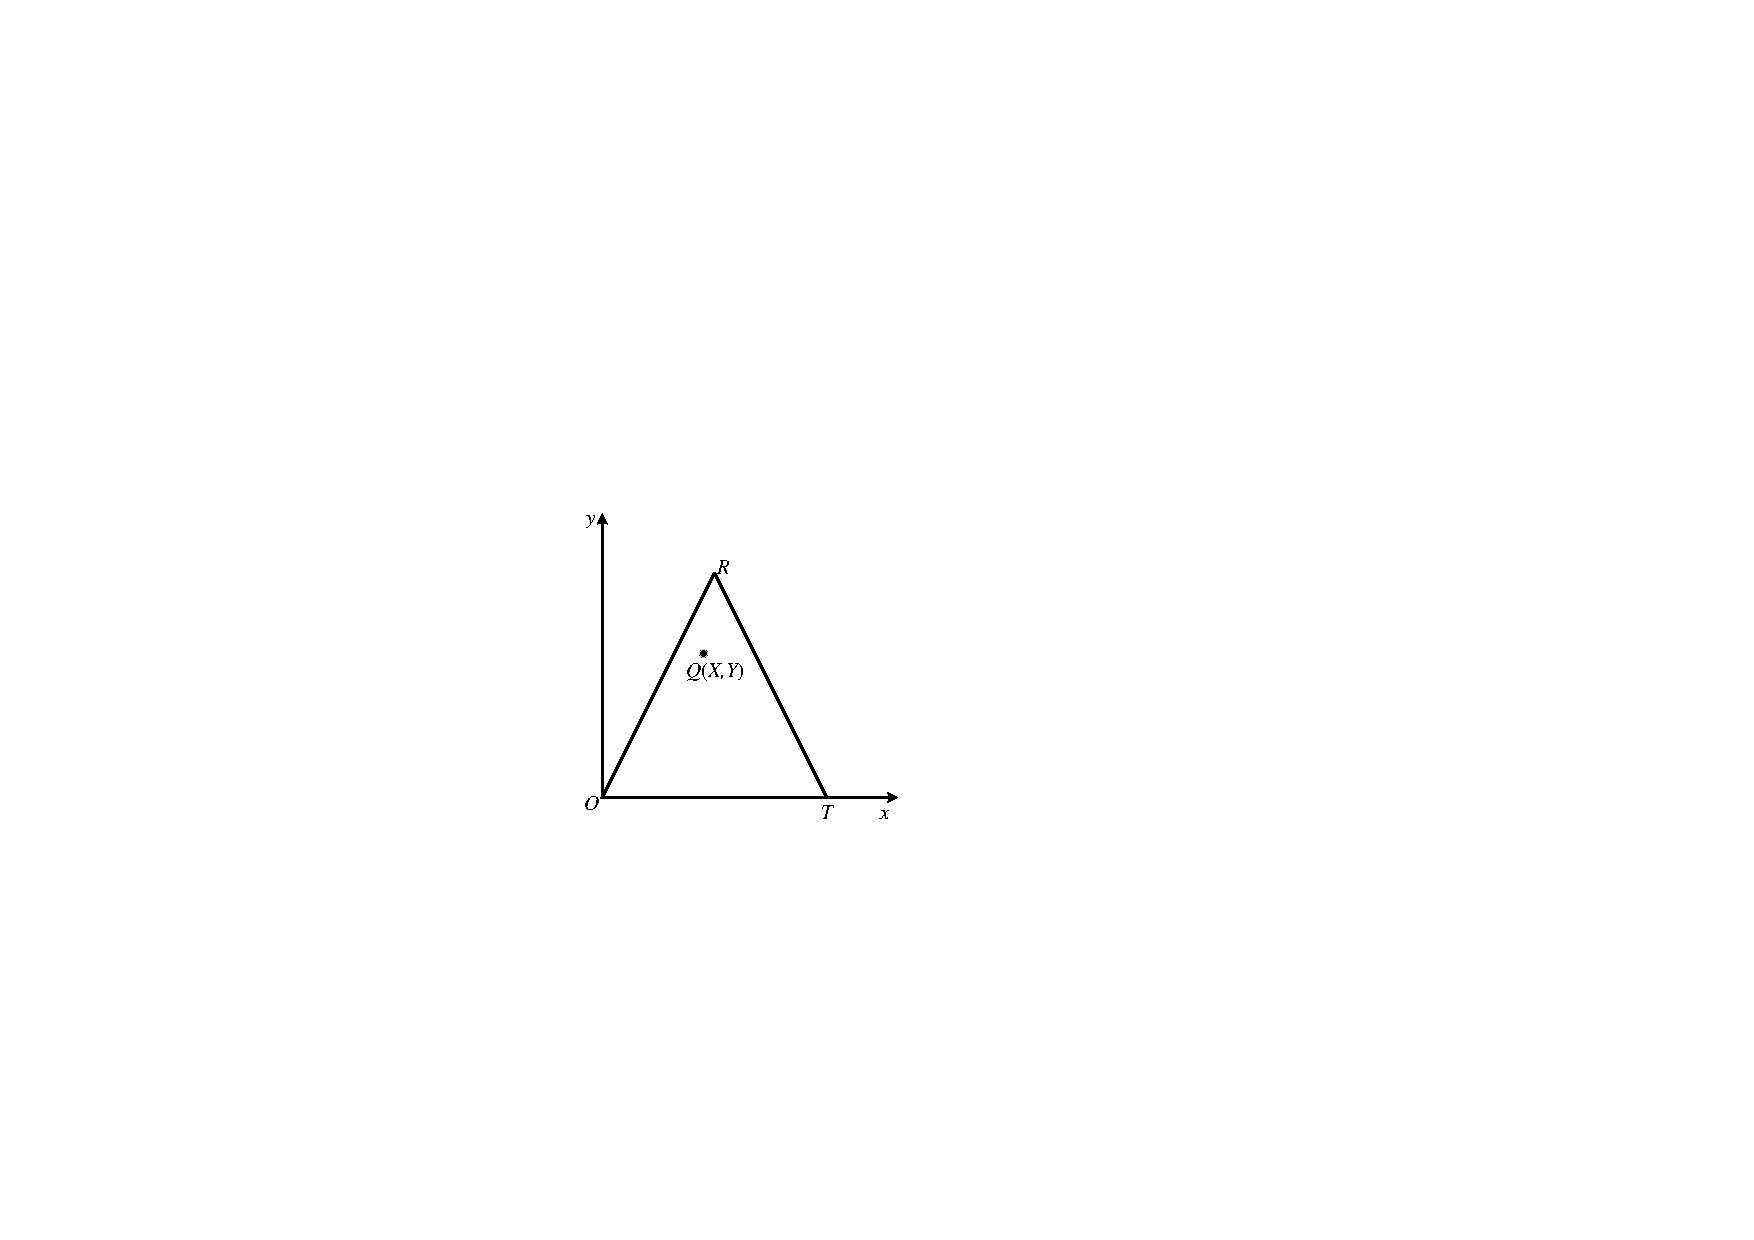
\includegraphics[width=0.2\textwidth]{25.pdf}
    % \end{figure}
    % \vspace{-0.5cm}




    \item 一打靶场备有5支某种型号的枪,其中3支已经校正,2支未经校正.某人使用已校正
    的枪击中目标的概率为$p_1$.使用未经校正的枪击中目标的概率为$p_2$.他随机地取一支枪进行
    射击,已知他射击了5次,都未击中,求他使用的是已校正的枪的概率(设各次射击的结果相
    互独立).



    \item 某人共买了11个水果,其中有3个是二级品,8个是一级品.随机地将水果分给$A,B,C$
    三人,各人分别得到4个、6个、1个.
    \begin{enumerate}
        \item 求$C$未拿到二级品的概率.
        \item 已知$C$未拿到二级品,求$A,B$均拿到二级品的概率.
        \item 求$A,B$均拿到二级品而$C$未拿到二级品的概率.
    \end{enumerate}



    \item 一系统$L$由两个只能传输字符0和1的独立工作的子系统$L_1$与$L_2$串联而成(如
    图),每个子系统输入为0输出为0的概率为$p(0<p<1)$;而输入为1输出为1的概率也是
    $p$.今在图中$a$端输入字符1,求系统$L$的$b$端输
    出字符0的概率.
    \begin{figure}[H]
        \flushright 
        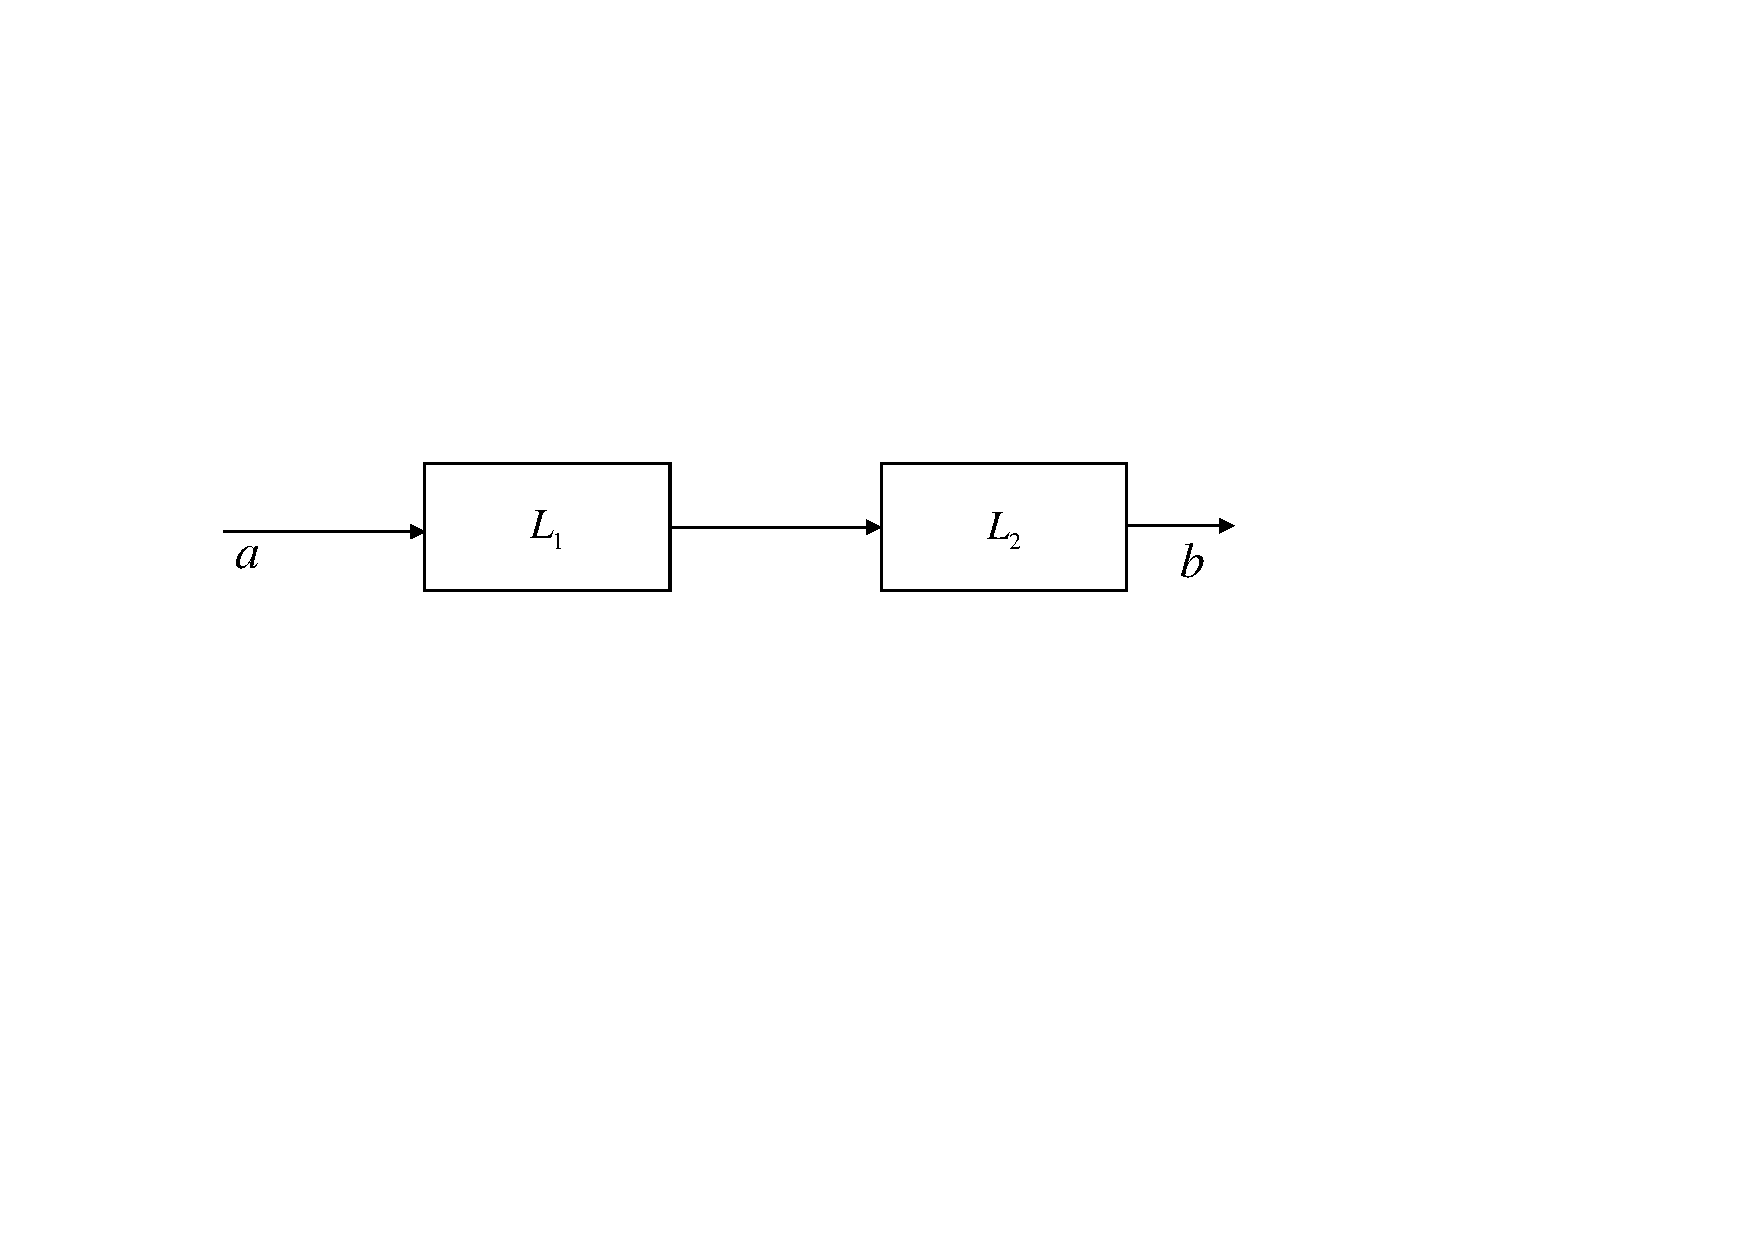
\includegraphics[width=0.4\textwidth]{3.pdf}
    \end{figure}
    \vspace{-0.5cm}



    \item 甲乙两人轮流掷一颗骰子,每轮掷一次,谁先掷得6点谁得胜,从甲开始掷,问甲、乙得胜的
    概率各为多少?



    \item 将一颗骰子掷两次,考虑事件: $A=\mbox{“第一次掷得点数2或5”}$.$B=\mbox{“两次点数之和至少为7”}$,
    求$P(A),P(B)$,并问事件$A,B$是否相互独立.



    \item $A,B$两人轮流射击,每次每人射击一枪,射击的次序为$A,B,A,B,A,\cdots$,射击直至击
    中两枪为止.设每人击中的概率均为$p$,且各次击中与否相互独立.求击中的两枪是由同一人
    射击的概率.(提示:分别考虑两枪是由$A$击中的与两枪是由$B$击中的两种情况,若两枪是由
    $A$击中的,则射击必然在奇数次结束.又当$|x|<1$时,$1+2x+3x^2+\cdots=1/(1-x)^2$.)


    \item 有3个独立工作的元件1,元件2,元件3,它们的可靠性分别为$p_1,p_2,p_3$.设由它们组
    成一个“3个元件取2个元件的表决系统”,记为$2/3[G]$. 这一系统的运行方式是当且仅当3个元件中至少有2个正
    常工作时这一系统正常工作.求这一$2/3[G]$系统的可靠性.



    \item 在如图所示的桥式结构的电路中,第$i$个继电器触点闭合的概率为$p_i,i=1,2,3,4,5$.各继电器工作相互
    独立,求:
    \begin{figure}[H]
        \flushright 
        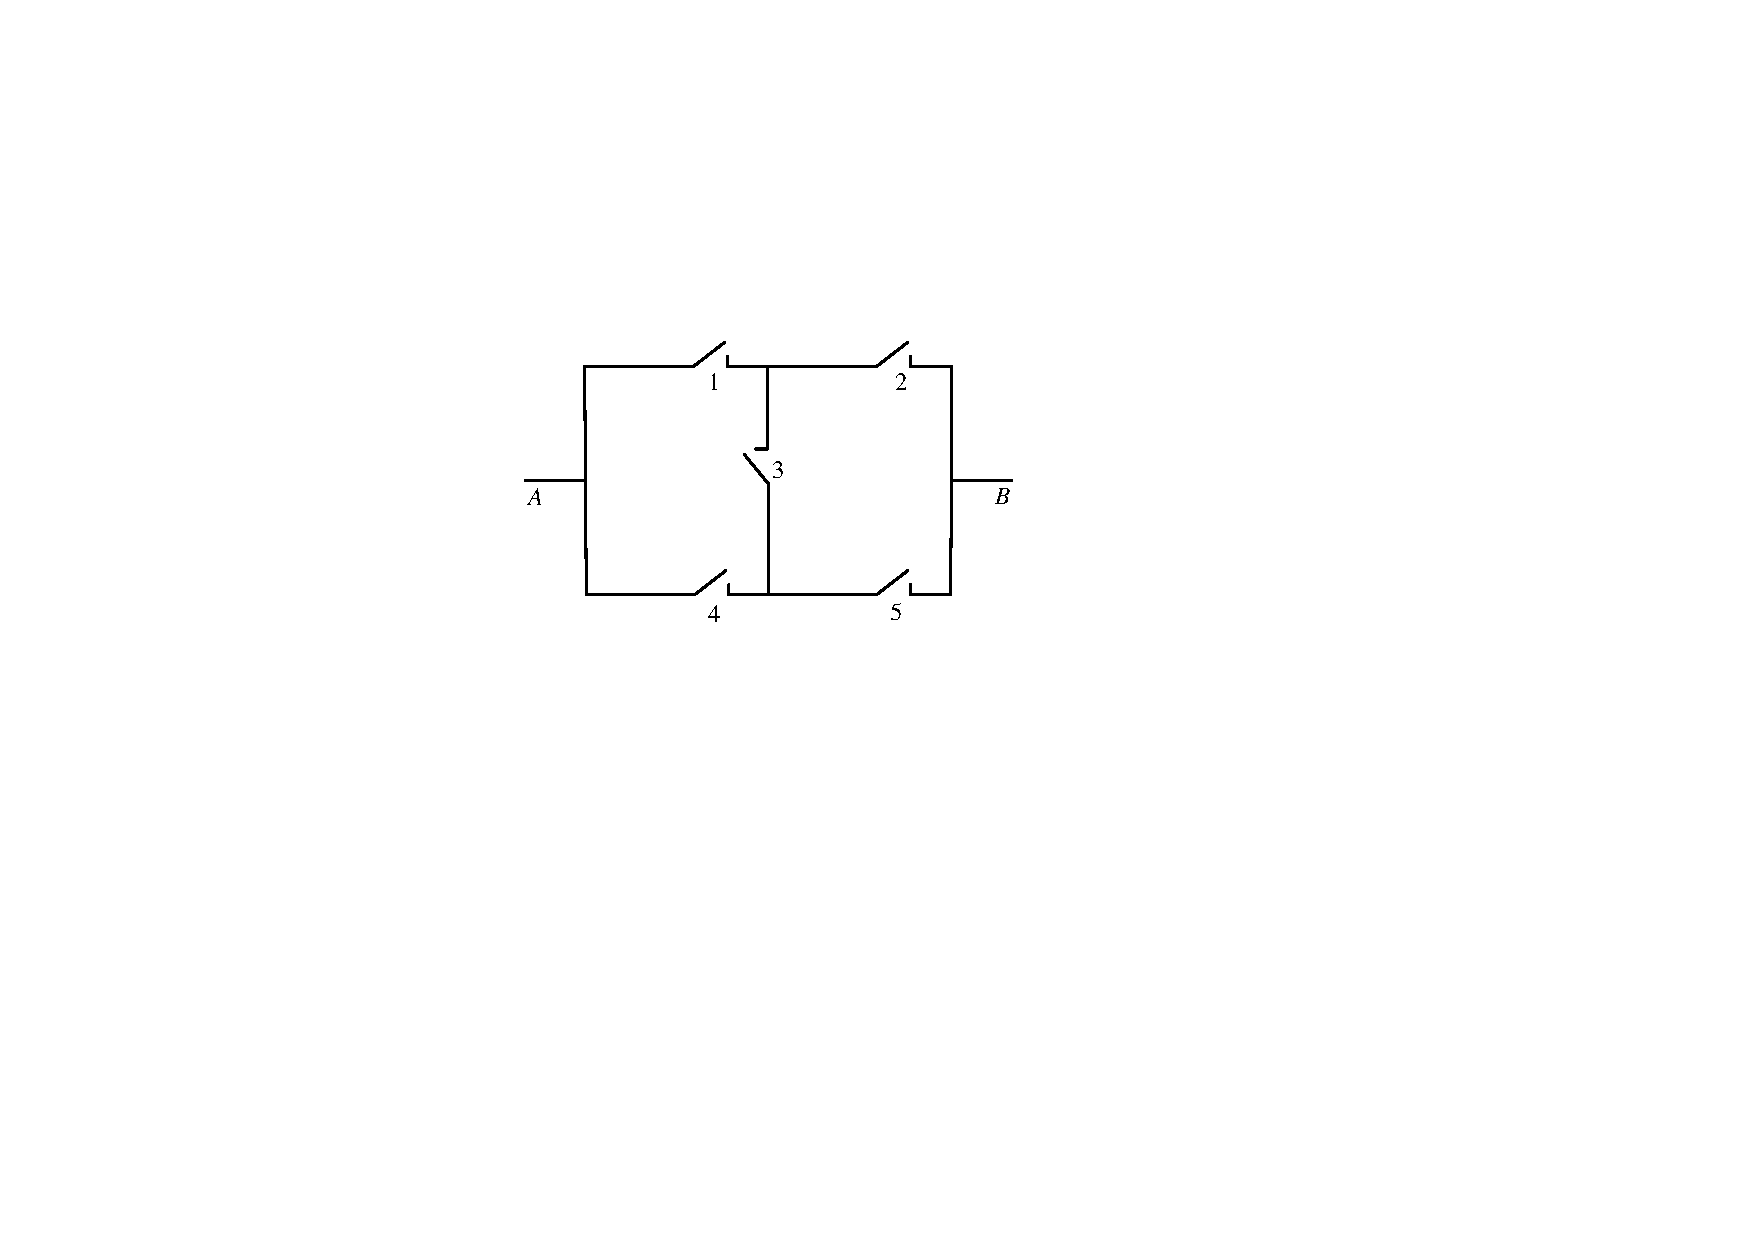
\includegraphics[width=0.25\textwidth]{8.pdf}
    \end{figure}
    \vspace{-0.5cm}
    \begin{enumerate}
        \item 以继电器触点1是否闭合为条件,求$A$到$B$之间为通路的概率.
        \item 已知$A$到$B$为通路的条件下,继电器触点3是闭合的概率.
    \end{enumerate}


    \item 进行非学历考试,规定考甲、乙两门课程,每门课程考试第一次未通过都只允许考第二
    次.考生仅在课程甲通过后才能考课程乙.如两门课程都通过可获得一张资格证书.设某考生
    通过课程甲的各次考试的概率为$p_1$,通过课程乙的各次考试的概率为$p_2$,设各次考试的结果
    相互独立.又设考生参加考试直至获得资格证书或者不准予再考为止.以$X$表示考生总共需
    考试的次数.求$X$的分布律.


    \item \begin{enumerate}
        \item 5只电池,其中有2只是次品,每次取一只测试,直到将2只次品都找到.设第
        2只次品在第$X(X=2,3,4,5)$次找到,求$X$的分布律(注:在实际上第5次检测可无需进
        行).
        \item 5只电池,其中2只是次品,每次取一只,直到找出2只次品或3只正品为止.写出需
        要测试的次数的分布律.
    \end{enumerate}



    \item 


    


    

    

  

\end{enumerate}
\end{document}